\documentclass[a4paper]{article}
\usepackage[T1,T2A]{fontenc}
\usepackage[utf8]{inputenc}
\usepackage[english,russian]{babel}
\usepackage{booktabs}
\usepackage{color,colortbl}
%\usepackage{amsmath}
%\usepackage{amsfonts}
%\usepackage{amssymb}
%\usepackage{makeidx}
\usepackage{listings}
\usepackage{graphicx}
\usepackage{rotating}
\definecolor{green}{RGB}{45,140,31}
\definecolor{darkishgreen}{RGB}{39,203,22}
\definecolor{LightCyan}{rgb}{0.88,1,1}
\definecolor{Gray}{gray}{0.9}
\definecolor{lightRed}{RGB}{230,170,150}
\definecolor{modRed}{RGB}{230,82,90}
\definecolor{strongRed}{RGB}{230,6,6}

\lstset{ %
  language=SQL,                % Язык программирования
  numbers=left,                   % С какой стороны нумеровать
  extendedchars=\true,
  %numberstyle=tinycolor{gray},     % Стиль который будет использоваться для нумерации строк
  %stepnumber=2,                   % Шаг между линиями. Если 1, то будет пронумерована каждая строка
 % numbersep=5pt,
 % backgroundcolor=color{white},      % Цвет подложки. Вы должны добавить пакет color - usepackage{color}
  showspaces=false,
  showstringspaces=false,
  showtabs=false,
  %frame=single,                    % Добавить рамку
  %rulecolor=color{black},
  tabsize=4,                       % Tab - 2 пробела
  breaklines=true,                 % Автоматический перенос строк
  breakatwhitespace=true,          % Переносить строки по словам
  title=lstname,                   % Показать название подгружаемого файла
  keywordstyle=\color{green},          % Стиль ключевых слов
  %commentstyle=color{dkgreen},       % Стиль комментариев
  %stringstyle=color{mauve}          % Стиль литералов
}

\usepackage[english,russian]{babel}

\begin{document}

\begin{titlepage}
  \newpage
  \begin{center}
    {\bfseries Сарапульский политехнический институт (филиал)
      федерального государственного бюджетного образовательного
      учреждение высшего образования
      «Ижевский государственный технический университет имени М.Т. Калашникова» \linebreak
      (СПИ (филиал) ФГБОУ ВО «ИжГТУ имени \linebreak
      М.Т. Калашникова»)
    }
  \end{center}
    \begin{center}
      % \textsc{\textbf{}}
      \topskip=0pt
      \vspace*{\fill}
      \large \textbf{Информационные технологии} \linebreak
      методические указания к выполнению лаборатрных работ \linebreak
      для студентов направления 20.03.01 \linebreak
      «Техносферная безопасность» \linebreak
      для всех форм обучения 
      \vspace*{\fill}
    \end{center}
    \begin{center}
      Составитель:
      \hspace*{\fill} старший преподаватель \linebreak
      \hspace*{\fill} Романцов Г. Д.
    \end{center}
     \begin{center}
       \vspace*{\fill}
       Сарапул\linebreak 2020
    \end{center}
  \end{titlepage}

  \tableofcontents
  \newpage
  \documentclass[a4paper]{article}
\usepackage[T1,T2A]{fontenc}
\usepackage[utf8]{inputenc}
\usepackage[english,russian]{babel}
\usepackage{booktabs}
\usepackage{color,colortbl}
%\usepackage{amsmath}
%\usepackage{amsfonts}
%\usepackage{amssymb}
%\usepackage{makeidx}

\definecolor{darkishgreen}{RGB}{39,203,22}
\definecolor{LightCyan}{rgb}{0.88,1,1}
\definecolor{Gray}{gray}{0.9}
\definecolor{lightRed}{RGB}{230,170,150}
\definecolor{modRed}{RGB}{230,82,90}
\definecolor{strongRed}{RGB}{230,6,6}

\usepackage[english,russian]{babel}

\begin{document}

\section{Лабораторная работа. Операции с двоичными числами}

Цель работы:

\subsection{Теоретические основы}

В основу работы ЭВМ положены арифметические и логические операции с двоичными числами. Правила выполнения арифметических действий над двоичными числами можно представить таблицами сложения, вычитания и умножения. Все действия в двоичной арифметике сводятся к поразрядному выполнению трёх указанных операций в таблице~\ref{tab:mytab}.

Правила арифметики во всех позиционных системах счисления аналогичны. В двоичной системе арифметическое сложение происходит так же, как в десятичной системе с учетом переноса единицы в старший разряд.

\begin{table}[h]
  \caption{Арифметические действия над двоичными числамин}
  \begin{center}\label{tab:mytab}
   \begin{tabular}{c|c|c}
     Сложение & Вычитание & Умножение \\
     $0 + 0 = 0$ & $0 - 0 = 0$ & $0 * 0 = 0$\\
     $0 + 1 = 1$ & $0 - 1 = -11$ & $0 * 1 = 0$\\
     $1 + 0 = 1$ & $1 - 1 = 1$ & $1 * 0 = 0$\\
     $1 + 1 = 10$ & $1 - 1 = 0$ & $1 * 1 = 1$\\
     \end{tabular}
  \end{center}       
\end{table}

\begin{center}

Пример 1. Выполнить операцию арифметического сложения.
\[
\begin{array}{r}
+
\begin{array}{r}
01101\\
00111\\
\end{array} \\
\midrule
\begin{array}{r}
10100
\end{array}
\end{array}
\]
Пример 2. Выполнить операцию арифметического вычитания.
\[
\begin{array}{r}
-
\begin{array}{r}
01101\\
00111\\
\end{array} \\
\midrule
\begin{array}{r}
00110
\end{array}
\end{array}
\]
Пример 3. Выполнить операцию арифметического умножения.

\[
\begin{array}{r}
*
\begin{array}{r}
0001101\\
0000111\\
\end{array} \\
\midrule
\begin{array}{r}
1011011
\end{array}
\end{array}
\]

\end{center}

Следует заметить, что в реальных ЭВМ чаще всего используются 16-, 32-, 64-разрядные сетки (машинные слова). Однако для учебных целей рассматривается простой вариант выполнения операции сложения.


Очень часто в вычислениях должны использоваться не только положительные, но и отрицательные числа. Число со знаком в вычислительной технике представляется путем представления старшего разряда числа в качестве знакового. Принято считать, что 0 в знаковом разряде означает знак «плюс» для данного числа, а 1 – знак «минус». Выполнение арифметических операций над числами с разными знаками представляется для аппаратной части довольно сложной процедурой. В этом случае нужно определить большее по модулю число, произвести вычитание и присвоить разности знак большего по модулю числа. Применение дополнительного кода позволяет выполнить операцию алгебраического суммирования и вычитания на обычном сумматоре. При этом не требуется определения модуля и знака числа. \linebreak
\textbf{Прямой код} пyредставляет собой одинаковое представление значимой части числа для положительных и отрицательных чисел и отличается только знаковым битом. В прямом коде число 0 имеет два представления «+0» и «–0». \linebreak
\textbf{Обратный код} для положительных чисел имеет тот же вид, что и прямой код, а для отрицательных чисел образуется из прямого кода положительного числа путем инвертирования всех значащих разрядов прямого кода. В обратном коде число 0 также имеет два представления «+0» и «–0». \linebreak
\textbf{Дополнительный код} для положительных чисел имеет тот же вид, что и прямой код, а для отрицательных чисел образуется путем прибавления 1 к обратному коду. Добавление 1 к обратному коду числа 0 дает единое представление числа 0 в дополнительном коде. Однако это приводит к асимметрии диапазонов представления чисел относительно нуля. Так, в восьмиразрядном представлении диапазон изменения чисел с учетом знака. \linebreak

\[-128 <= x <= 127\]

\subsubsection{Сложение и вычитание чисел со знаком в дополнительном коде}

В ЭВМ вычитание заменяется сложением чисел в обратном или в дополнительном коде, что позволяет и для вычитания и для сложения использовать одно и тожк устройство --- сумматор.

При вычитании чисел при помощи обратного кода, после операции сложения в обратном коде получается промежуточный результат, к которому нужно прибавить значение разряда переноса, после чего отбросить этот разряд.

В дополнительном коде в отличие от обратного возможный перенос учитывается в самих числах, а не в результате. После операциисложения в дополнительном коде получается промежуточный результат, от которого нужно отбросить разряд переноса.

\begin{table}
      \caption{Пример сложение чисел в двоичной системе счисления}
      \begin{center}\label{tab:add}
      \begin{tabular}{c * {11}{c}}
        \toprule
        Номер бита & Перенос 8 & 7 & 6 & 5 & 4 & 3 & 2 & 1 & 0 \\
        \toprule
        Число А ($43 = 32 + 8 + 2 + 1$) &  & 0 & 0 & 1 & 0 & 1 & 0 & 1 & 1\\
        \midrule
        Число B ($29 = 16 + 8 + 4 + 1$) &  & 0 & 0 & 0 & 1 & 1 & 1 & 0 & 1\\
        \midrule
        Перенос из разряда &  &  & 1 & 1 & 1 & 1 & 1 & 1 & \\
        \midrule
        Сумма ($72 = 43 + 29$) &  & 0 & 1 & 0 & 0 & 1 & 0 & 0 & 0 \\
        \bottomrule
      \end{tabular}
    \end{center}
\end{table}


\begin{table}
      \caption{Пример вычитания в двоичной системе счисления с использованрием обратного кода}
      \begin{center}\label{tab:sub_OB}
        %\toprule
      \begin{tabular}{c * {11}{c}}
        \toprule
        Номер бита & Перенос 8 & 7 & 6 & 5 & 4 & 3 & 2 & 1 & 0 \\
        \toprule
        Модуль числа 29 ($29 = 16 + 8 + 4 + 1$) &  & 0 & 0 & 0 & 1 & 1 & 1 & 0 & 1\\
        \midrule
        Обратый код числа 29 ($29 = 16 + 8 + 4 + 1$) &  & 1 & 1 & 1 & 0 & 0 & 0 & 1 & 0\\
        \midrule
        Число А ($43 = 32 + 8 + 2 + 1$) &  & 0 & 0 & 1 & 0 & 1 & 0 & 1 & 1\\
        \midrule
        Перенос из разряда &  &  & 1 &  &  &  & 1 &  & \\
        \midrule
        Сумма (промежуточный результат) & 1 & 0 & 0 & 0 & 0 & 1 & 1 & 0 & 1 \\
        \midrule
        + перенос &  &  &  &  &  &  &  &  & 1 \\
        \midrule
        Сумма (окончательный результат) &  & 0 & 0 & 0 & 0 & 1 & 1 & 1 & 0 \\
        \bottomrule
      \end{tabular}
    \end{center}
\end{table}

\begin{table}
      \caption{Пример вычитания в двоичной системе счисления с использованрием дополнительного кода}
      \begin{center}\label{tab:sub_DP}
        %\toprule
      \begin{tabular}{c * {11}{c}}
        \toprule
        Номер бита & Перенос 8 & 7 & 6 & 5 & 4 & 3 & 2 & 1 & 0 \\
        \toprule
        Модуль числа 29 ($29 = 16 + 8 + 4 + 1$) &  & 0 & 0 & 0 & 1 & 1 & 1 & 0 & 1\\
        \midrule
        Обратый код числа 29 ($29 = 16 + 8 + 4 + 1$) &  & 1 & 1 & 1 & 0 & 0 & 0 & 1 & 0\\
        \midrule
        +1 ($29 = 16 + 8 + 4 + 1$) &  &  &  &  &  &  &  &  & 1\\
        \midrule
        Дополнительный код числа 29 ($29 = 16 + 8 + 4 + 1$) &  & 1 & 1 & 1 & 0 & 0 & 0 & 1 & 1\\
        \midrule
        Число А ($43 = 32 + 8 + 2 + 1$) &  & 0 & 0 & 1 & 0 & 1 & 0 & 1 & 1\\
        \midrule
        Перенос из разряда &  & 1 & 1 &  &  &  & 1 & 1 & \\
        \midrule
        Сумма (промежуточный результат) & 1 & 0 & 0 & 0 & 0 & 1 & 1 & 1 & 0 \\
        \midrule
        + перенос &  &  &  &  &  &  &  &  & 1 \\
        \midrule
        Сумма (окончательный результат) &  & 0 & 0 & 0 & 0 & 1 & 1 & 1 & 0 \\
        \bottomrule
      \end{tabular}
    \end{center}
\end{table}

\newpage
\subsection{Задание на лабораторную работу}

Для выполнения работы необходимо:
\begin{enumerate}
  \item Изучить теоретический материал
  \item Из таблицы~\ref{tab:tasks} выбрать числовые данные в соответствии с вашим вариантом.
  \item Перевести десячичные числа в двоичные
  \item Выполнить указанные операции над ними ()
  \item Записать решения по примеру таблиц~\ref{tab:add},~\ref{tab:sub_OB},~\ref{tab:sub_DP}
    \item Оформить отчет по лабораторной работе
\end{enumerate}

\begin{table}[h]
      \caption{Варианты заданий}
      \begin{center}\label{tab:tasks}
        %\toprule
      \begin{tabular}{|c|cccccc|}
        \hline
        Вариант & 1 & 2 & 3 & 4 & 5 & 6\\
        \hline
        1 & 2+2 & 34+32 & 6-4 & 64-32 & 89-23 & 10-40\\
        \hline
        2 & 2+3 & 12+64 & 6-2 & 23-12 & 128-89 & 15-31\\
        \hline
        3 & 4+7 & 14+65 & 4-2 & 54-23 & 100-78 & 16-32\\
        \hline
        4 & 3+5 & 15+32 & 4-1 & 56-44 & 90-32 & 2-19\\
        \hline
        5 & 5+3 & 44+12 & 10-3 & 78-34 & 123-120 & 15-16\\
        \hline
        6 & 6+9 & 8+21 & 3-1 & 79-45 & 111-11 & 31-32\\
        \hline
        7 & 6+4 & 12+21 & 4-1 & 79-10 & 111-100 & 54-63\\
        \hline
        8 & 7+2 & 56+22 & 5-2 & 39-14 & 128-28 & 22-64\\
        \hline
        9 & 9+3 & 23+32 & 6-5 & 55-22 & 120-30 & 23-88\\
        \hline
        10 & 4+7 & 45+32 & 9-3 & 88-22 & 90-8 & 16-31\\
        \hline
        11 & 3+4 & 32+32 & 8-2 & 44-21 & 123-33 & 32-63\\
        \hline
        12 & 3+2 & 64+16 & 10-5 & 78-67 & 129-88 & 15-38\\
        \hline
        13 & 4+5 & 16+32 & 10-2 & 81-64 & 148-64 & 44-88\\
        \hline
        14 & 7+7 & 23+24 & 2-1 & 64-16 & 63-15 & 57-78\\
        \hline
        15 & 5+5 & 54+40 & 7-5 & 55-12 & 120-15 & 76-100\\
        \hline
        16 & 6+6 & 41+23 & 7-3 & 65-15 & 115-31 & 55-105\\
        \hline
      \end{tabular}
    \end{center}
\end{table}
                                     
\newpage
\subsection{Содержание отчета}
\begin{enumerate}
  \item Титульный Лист
  \item Цель работы
  \item Краткие теоретические сведения по теме лабораторной работы
  \item выполненное задание
  \item краткий вывод о проделанной работе
\end{enumerate}

\subsection{Литература}


\end{document}

  \newpage
  %\documentclass[a4paper]{article}
%\usepackage[T1,T2A]{fontenc}
%\usepackage[utf8]{inputenc}
%\usepackage[english,russian]{babel}
%\usepackage{booktabs}
%\usepackage{color,colortbl}
%\usepackage{amsmath}
%\usepackage{amsfonts}
%\usepackage{amssymb}
%\usepackage{makeidx}
%\usepackage{tikz}
%\usetikzlibrary{graphs}
%\usepackage{graphicx}
%\definecolor{darkishgreen}{RGB}{39,203,22}
%\definecolor{LightCyan}{rgb}{0.88,1,1}
%\definecolor{Gray}{gray}{0.9}
%\definecolor{lightRed}{RGB}{230,170,150}
%\definecolor{modRed}{RGB}{230,82,90}
%\definecolor{strongRed}{RGB}{230,6,6}

%\usepackage[english,russian]{babel}

%\begin{document}


\section{Лабораторная работа №2.\newline Системы счисления}

Цель работы:
\begin{enumerate}
    \item Понять принципы позиционной системы счисления.
    \item Научиться переводить числа из одной системы в другую.
    \item Уметь производить арифметические действия над числами, представленными в различных системах счисления.
\end{enumerate}

\subsection{Теоретические основы}

Под системой счисления принято понимать совокупность приемов записи чисел. Условные знаки, которые при этом применяются, называют цифрами. В некоторых системах счисления кроме цифр могут использоваться специальные символы. Таким образом, в системах счисления числа записываются как последовательность цифр или специальных символов. Системы счисления подразделяются на позиционные и непозиционные. В непозиционной системе счисления значение цифры не зависит от ее положения в записи числа. К непозиционной системе счисления относится, так называемая, Римская система счисления. Например, возьмем число XXX из Римской системы счисления. В данном числе цифра X в любом месте означает число десять. В позиционных системах счисления значение каждой цифры зависит от ее положения (позиции) в ряду цифр, изображающих это число. Например. В числе 999 (десятичная система счисления) первая справа цифра 9 означает количество единиц, содержащихся в числе, вторая - количество десятков, третья - количество сотен. Принимая за основание системы различные числа можно получить соответствующие системы счисления. Число Рединиц одного разряда, объединяемых в единицу более старшего разряда, называют основанием позиционной системы счисления, а сама система называется Р-ичной. Поэтому для записи произвольного числа в какой-либо позиционной системе счисления достаточно иметь Р различных цифр. Таким образом, любая позиционная система с любым целым основанием P (при P>1) использует Р различных цифр а, которые обозначают последовательный ряд чисел от 0 и кончая числом Р-1.

Число записывается в виде последовательности Р-ичных цифр, которая разделена точкой на целую и дробную части. Если каждый из символов $а_{n}, a_{n-1},\dots,a_{1}, a_{0}, a_{-1}, \dots,a_{m}$ означает некоторую Р-ичную цифру, то запись числа имеет вид $а_{n}, a_{n-1},\dots,a_{1}, a_{0},a_{-1}, \dots,a_{m}$. Каждой цифре из этой последовательности принято определенное значение. Цифра, стоящая в некотором разряде, имеет значение в Р раз большее того, которое она имела бы в разряде с номером, меньшим на
1. И наоборот, в Р раз меньше того, которое она имела бы в разряде с номером, большим на 1.

\subsubsection{Позиционные системы счисления}

Как было сказано, количество различных цифр, применяемых в позиционной системе счисления, называют ее основанием. Принимая за основание системы различные числа можно получить соответствующие системы счисления. К позиционной системе счисления, получившим наибольшее распространение, относятся десятичная, двоичная, восьмеричная и шестнадцатеричная системы счисления. Для того, чтобы отличать в какой системе представлено то или иное число, в дальнейшем будем записыватьчисло с указанием используемой системы счисления. Например, 375ю - число 375 в десятичной системе счисления, а число 3758 - число 375 в восьмеричной системе счисления.

\textbf{Десятичная система счисления}

Это наиболее широко распространенная система счисления, которая использует 10 различных базисных цифр для представления любой величины. При записи чисел в десятичной системе счисления используются символы 0, 1, 2, 3, 4, 5, 6, 7, 8, 9.

Несмотря на простоту и привычность десятичной системы счисления, использование ее при передачи информации в вычислительных машинах представляется неудобной и технически не экономичной. Поэтому при организации вычислительных процессов в ЭВМ используются системы счисления с другими основаниями.

\textbf{Двоичная система счисления}

Большинство элементов, из которых строится ЭВМ, по своей физической природе могут находиться лишь в одном из двух состояний. Такие элементы называются двухпозиционными. Одно из устойчивых состояний элемента принимается за изображение цифры 0, а другое за изображение цифры 1. С помощью двухпозиционных элементов легко изображаются разряды двоичного числа. Поэтому двоичная система счисления имеет преимущества, и она оказывается очень удобной для применения в ЭВМ. Двоичная система счисления имеет только две цифры: 0 и 1. Это минимальное количество цифр, которое может быть принято в системе счисления. Как и в десятичной системе счисления, в двоичной системе для отделения дробной части от целой используется точка, а перед отрицательным числом ставиться минус (-): $101.1_{2}, 1.001_{2}, -101_{2}$.

\textbf{Восьмеричная система счисления}

В цифровых схемах и электронных системах получила распространение восьмеричная система счисления. Данная система удобна тем, что восьмеричная запись какого-либо числа в три раза короче его двоичной записи. В данной системе счисления коэффициенты принимают восемь различных значений - 0, 1, 2, 3, 4, 5, 6, 7.
Поэтому каждый восьмеричный символ может быть представлен трехбитовым числом. Этих чисел восемь, как и символов в восьмеричной системе счисления. Как и в рассмотренных системах счисления, в восьмеричной системе используются дробные и отрицательные числа: $7.35_{8},- 5.001_{8}, 345.67_{8}$.

\textbf{Шестнадцатеричная система счисления}

Для систем счисления с основанием больше «10», арабских цифр для представления чисел не хватит. Поэтому в этих случаях дополнительно вводят специальные символы. К таким системам счисления относится шестнадцатеричная система счисления.В шестнадцатеричной системе счисления используют 16 базисных символов: 0, 1, 2, 3, 4, 5, 6, 7, 8, 9, А, В, С, D, Е, F. Выбор шестнадцатеричной системы счисления обуславливается что эту систему можно использовать как средство сокращенной записи четырехзначного двоичного числа. Следует помнить, что шестнадцатеричные и восьмеричные числа - это только способ представления двоичных чисел. Для представления дробных чисел и отрицательных шестнадцатеричных чисел используется, соответственно, точка и знак минуса (-): $-AB_{16}; 1036.F_{16};FF.13_{16}$.

\subsubsection{Перевод чисел в позиционных системах счисления}

Для перевода целого десятичного числа в другую систему счисления, необходимо разделить исходное число на основание системы счисления, в которое оно переводится. При этом надо определять остатки от деления. Остаток первого деления является значением младшего разряда. Затем полученное частное делится на выбранное основание. Процедуру деления продолжают до тех пор, пока частное не станет меньше делителя, т.е. основания системы счисления, в которую осуществляется перевод. Значение последнего частного будет наибольшим разрядом, т.е. запись нового числа производится в обратном порядке: от частного к первому остатку, используя все промежуточные остатки. При переводе в шестнадцатеричную систему счисления остатки, значения которых больше 9, необходимо заменить соответствующими буквенным эквивалентом: 10 - А, 11 - В, 12 - С, 13 - D, 14 -Е, 15 -F.

Пример перевода десятичного числа 95:

В двоичную систему счисления $95_{10}=1011111_{2}$
\begin{figure}[h]
\center{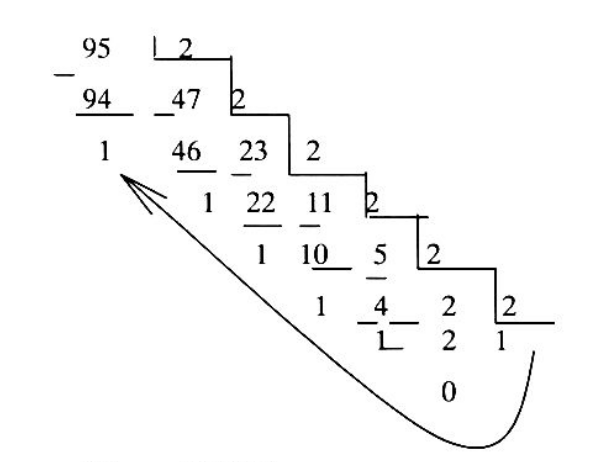
\includegraphics[width=128pt]{dectobin.png}
  \label{ris:dectobin}}
\end{figure}

В восьмиричную систему счисления $95_{10}=137_{8}$
\begin{figure}[h]
\center{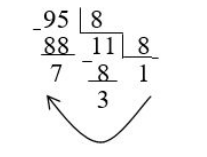
\includegraphics[width=64pt]{dectooct.png}
  \label{ris:dectooct}}
\end{figure}

В шестнадцатиричную систему счисления $95_{10}=5F_{16}$
\begin{figure}[h]
\center{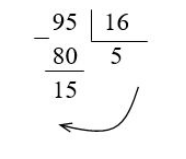
\includegraphics[width=64pt]{dectohex.png}
  \label{ris:dectohex}}
\end{figure}

При переводе правильных десятичных дробей, необходимо умножить значение этой дроби на основание системы счисления, в которую осуществляется перевод. Значение целой части результата первого умножения присваивается старшему разряду дробной части. Затем целая часть не рассматривается и производится следующее умножение дробной части. Процедуру умножения повторяют до тех пор, пока результат умножения не будет равен целому числу и этот результат будет младшим разрядом, либо не будет достигнута требуемая точность.

Пример перевода десятичного числа 0.36:

В двоичную систему счисления $0.36_{10}=0.0101_{2}$
\begin{figure}[h]
\center{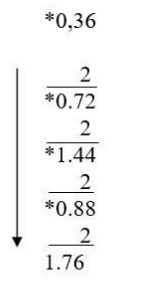
\includegraphics[width=64pt]{fdectobin.png}
  \label{ris:fdectobin}}
\end{figure}

В восьмиричную систему счисления $0.36_{10}=0.2702_{8}$

\begin{figure}[h]
\center{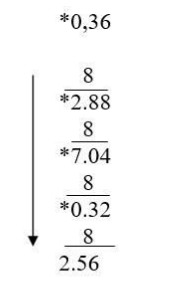
\includegraphics[width=64pt]{fdectooct.png}
  \label{ris:fdectooct}}
\end{figure}

В шестнадцатиричную систему счисления $0.36_{10}=0.5C28_{16}$

\begin{figure}[h]
\center{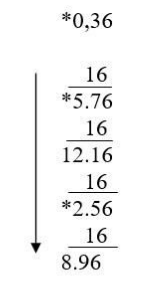
\includegraphics[width=64pt]{fdectohex.png}
  \label{ris:fdectohex}}
\end{figure}

Для перевода неправильной десятичной дроби, необходимо перевести отдельно дробную и целую часть, а полученные результаты сложить. Например, перевести в двоичную систему счисления неправильную десятичную дробь 14.375.
$$14_{10}=1110_{2} 0.375_{10}=0.011_{2} 14.375_{10}=1110.011_{2}$$

\subsubsection{Перевод в десятичную систему счисления}
Для перевода из любой позиционной системы счисления в десятичную систему счисления необходимо записать это число в виде суммы:
$$x = \sum^{n+m}_{i=1}(a_{i}*p^{n-i})$$
где Р --- основание системы из которой осуществляется перевод;\newline
а --- число, соответствующее базисной цифре Р-ичной системы счисления;\newline
n --- число цифр в целой части, m - число цифр в дробной части.\newline
Например, перевести число $110.101_{2}$ из двоичной системы счисления в десятичную:
$$110.101_{2} = 1 * 2^{2} + 1 * 2^{1} + 0 + 1 * 2^{-2} + 1 * 2^{-3} = 6.625_{10}$$

\subsubsection{Перевод из двоичной системы счисления в восьмеричную и шестнадцатеричную}

Основания восьмеричной и шестнадцатеричной систем счисления (q) являются степенью двоичной системы $(р):q=p$, где к --- целое число, равное 3 для восьмеричной системы счисления и 4 для шестнадцатеричной. Поэтому перевод из двоичной системы осуществляется разбиением двоичного числа на группы по три цифры в каждой для восьмеричной и по четыре для шестнадцатеричной. Отчет ведется от точки разделяющей целую часть от дробной в обе стороны. Затем каждая группа заменяется соответствующей цифрой из соответствующих систем счисления(см. табл. \ref{tab:octhex}). Недостающие биты двоичного числа дополняются нулями: впереди - для целой части и в конце - для дробной части. Например, необходимо перевести двоичное число 1010001110.00111 в восьмеричное и шестнадцатеричное число:
\begin{itemize}
  \item в восьмеричное $1010001110.00111_{2} = 001 010 001 100.001 110_{2} = 1214.16_{8}$
  \item в шестнадцатеричное $1010001110.00111_{2} = 0010 1000 1100.0011 1000_{2} = 28С.38_{16}$
\end{itemize}

\begin{table}[h]
  \caption{Соответствие цифр в разных системах счисления}
  \begin{center}\label{tab:octhex}
    \begin{tabular}{|c|c|c|}
      \hline
     Символы & k - 3 & k - 4 \\
     \hline
      0 & 000 & 0000 \\
      1 & 001 & 0001 \\
      2 & 010 & 0010 \\
      3 & 011 & 0011 \\
      4 & 100 & 0100 \\
      5 & 101 & 0101 \\
      6 & 110 & 0110 \\
      7 & 111 & 0111 \\
      8 &     & 1000 \\
      9 &     & 1001 \\
      A &     & 1010 \\
      B &     & 1011 \\
      C &     & 1100 \\
      D &     & 1101 \\
      E &     & 1110 \\
      F &     & 1111 \\
      \hline
     \end{tabular}
  \end{center}
\end{table}

\subsubsection{Перевод в двоичную систему счисления из восьмеричной и шестнадцатеричной}
Для перевода в двоичную систему из восьмеричной или шестнадцатеричной системы счисления необходимо каждое число заменить двоичным эквивалентом (см. табл. \ref{tab:octhex}).

\subsubsection{Перевод из восьмеричной системы в шестнадцатеричную}
Для перевода из восьмеричной системы счисления в шестнадцатеричную систему счисления необходимо представить число в виде двоичного числа. Затем объединить в группы по 4 бита и заменить соответствующим числом из шестнадцатеричной системы счисления (см. табл. \ref{tab:octhex})

\subsubsection{Перевод из шестнадцатеричной системы в восьмеричную}
Для перевода из шестнадцатеричной системы счисления в восьмеричную необходимо представить число в виде двоичного числа. Затем объединить в группы по 3 бита и заменить соответствующим числом из восьмеричной системы счисления (см. табл. \ref{tab:octhex}).

\subsubsection{Арифметические действия в позиционных системах счисления}
Арифметические действия (сложение, вычитание, умножение и деление) над числами в восьмеричной и шестнадцатеричной системах счисления выполняются с использованием таблиц сложения и умножения подобно тому, как это делается в десятичной системе счисления. Таблицы \ref{tab:octsum} и \ref{tab:octmul} предназначены для выполнения сложения и умножения --- в восьмеричной системе счисления, а таблицы \ref{tab:hexsum} и \ref{tab:hexmul} - в шестнадцатеричной системе счисления. Ниже приведены примеры сложения и умножения в различных системах счисления.

\begin{table}[h]
  \caption{Сложение в восьмеричной системе}
  \begin{center}\label{tab:octsum}
\begin{tabular}{|c|c|c|c|c|c|c|c|}
  \hline
  + & 1 & 2 & 3 & 4 & 5 & 6 & 7\tabularnewline
\hline
1 & 2 & 3 & 4 & 5 & 6 & 7 & 10\tabularnewline
\hline
2 & 3 & 4 & 5 & 6 & 7 & 10 & 11\tabularnewline
\hline
3 & 4 & 5 & 6 & 7 & 10 & 11 & 12\tabularnewline
\hline
4 & 5 & 6 & 7 & 10 & 11 & 12 & 13\tabularnewline
\hline
5 & 6 & 7 & 10 & 11 & 12 & 13 & 14\tabularnewline
\hline
6 & 7 & 10 & 11 & 12 & 13 & 14 & 15\tabularnewline
\hline
7 & 10 & 11 & 12 & 13 & 14 & 15 & 16\tabularnewline
                                  \hline
\end{tabular}
\end{center}
\end{table}

\begin{table}[h]
  \caption{Умножение в восьмеричной системе}
  \begin{center}\label{tab:octmul}
\begin{tabular}{|c|c|c|c|c|c|c|c|}
\hline
{*} & 1 & 2 & 3 & 4 & 5 & 6 & 7\tabularnewline
\hline
1 & 1 & 2 & 3 & 4 & 5 & 6 & 7\tabularnewline
\hline
2 & 2 & 4 & 6 & 10 & 12 & 14 & 16\tabularnewline
\hline
3 & 3 & 6 & 11 & 14 & 17 & 22 & 25\tabularnewline
\hline
4 & 4 & 10 & 14 & 20 & 24 & 30 & 34\tabularnewline
\hline
5 & 5 & 12 & 17 & 24 & 31 & 36 & 43\tabularnewline
\hline
6 & 6 & 14 & 22 & 30 & 36 & 44 & 52\tabularnewline
\hline
7 & 7 & 16 & 25 & 34 & 43 & 52 & 61\tabularnewline
\hline
\end{tabular}
\end{center}
\end{table}

\begin{table}[h!]
  \caption{Сложение в шестнадцатеричной системе}
  \begin{center}\label{tab:hexsum}
\begin{tabular}{|c|c|c|c|c|c|c|c|c|c|c|c|c|c|c|c|}
\hline
+ & 1 & 2 & 3 & 4 & 5 & 6 & 7 & 8 & 9 & A & B & C & D & E & F\tabularnewline
\hline
1 & 2 & 3 & 4 & 5 & 6 & 7 & 8 & 9 & A & B & C & D & E & F & 10\tabularnewline
\hline
2 & 3 & 4 & 5 & 6 & 7 & 8 & 9 & A & B & C & D & E & F & 10 & 11\tabularnewline
\hline
3 & 4 & 5 & 6 & 7 & 8 & 9 & A & B & C & D & E & F & 10 & 11 & 12\tabularnewline
\hline
4 & 5 & 6 & 7 & 8 & 9 & A & B & C & D & E & F & 10 & 11 & 12 & 13\tabularnewline
\hline
5 & 6 & 7 & 8 & 9 & A & B & C & D & E & F & 10 & 11 & 12 & 13 & 14\tabularnewline
\hline
6 & 7 & 8 & 9 & A & B & C & D & E & F & 10 & 11 & 12 & 13 & 14 & 15\tabularnewline
\hline
7 & 8 & 9 & A & B & C & D & E & F & 10 & 11 & 12 & 13 & 41 & 15 & 16\tabularnewline
\hline
8 & 9 & A & B & C & D & E & F & 10 & 11 & 12 & 13 & 14 & 15 & 16 & 17\tabularnewline
\hline
9 & A & B & C & D & E & F & 10 & 11 & 12 & 13 & 14 & 15 & 16 & 17 & 18\tabularnewline
\hline
A & B & C & D & E & F & 10 & 11 & 12 & 13 & 14 & 15 & 16 & 17 & 18 & 19\tabularnewline
\hline
B & C & D & E & F & 10 & 11 & 12 & 13 & 14 & 15 & 16 & 17 & 18 & 19 & 1A\tabularnewline
\hline
C & D & E & F & 10 & 11 & 12 & 13 & 14 & 15 & 16 & 17 & 18 & 19 & 1A & 1B\tabularnewline
\hline
D & E & F & 10 & 11 & 12 & 13 & 14 & 15 & 16 & 17 & 18 & 19 & 1A & 1B & 1C\tabularnewline
\hline
E & F & 10 & 11 & 12 & 13 & 14 & 15 & 16 & 17 & 18 & 19 & 1A & 1B & 1C & 1D\tabularnewline
\hline
F & 10 & 11 & 12 & 13 & 14 & 15 & 16 & 17 & 18 & 19 & 1A & 1B & 1C & 1D & 1E\tabularnewline
\hline
\end{tabular}
\end{center}
\end{table}

\begin{table}[h!]
  \caption{Умножение в шестнадцатеричной системе}
  \begin{center}\label{tab:hexmul}
\begin{tabular}{|c|c|c|c|c|c|c|c|c|c|c|c|c|c|c|c|}
\hline
{*} & 1 & 2 & 3 & 4 & 5 & 6 & 7 & 8 & 9 & A & B & C & D & E & F\tabularnewline
\hline
1 & 1 & 2 & 3 & 4 & 5 & 6 & 7 & 8 & 9 & A & B & C & D & E & F\tabularnewline
\hline
2 & 2 & 4 & 6 & 8 & A & C & E & 10 & 12 & 14 & 16 & 18 & 1A & 1C & 1E\tabularnewline
\hline
3 & 3 & 6 & 9 & C & F & 12 & 15 & 18 & 1B & 1E & 21 & 24 & 27 & 2A & 2D\tabularnewline
\hline
4 & 4 & 8 & C & 10 & 14 & 18 & 1C & 20 & 24 & 28 & 2C & 30 & 34 & 38 & 3C\tabularnewline
\hline
5 & 5 & A & F & 14 & 19 & 1E & 23 & 28 & 2D & 32 & 37 & 3C & 41 & 46 & 4B\tabularnewline
\hline
6 & 6 & C & 12 & 18 & 1E & 24 & 2A & 30 & 36 & 3C & 42 & 48 & 4E & 54 & 5A\tabularnewline
\hline
7 & 7 & E & 15 & 1C & 23 & 2A & 31 & 38 & 3F & 46 & 4D & 54 & 5B & 62 & 69\tabularnewline
\hline
8 & 8 & 10 & 18 & 20 & 28 & 30 & 38 & 40 & 48 & 50 & 58 & 60 & 68 & 70 & 78\tabularnewline
\hline
9 & 9 & 12 & 1B & 24 & 2D & 36 & 3F & 48 & 51 & 5A & 63 & 6C & 75 & 7E & 87\tabularnewline
\hline
A & A & 14 & 1E & 28 & 32 & 3C & 46 & 50 & 5A & 64 & 6E & 78 & 82 & 8C & 96\tabularnewline
\hline
B & B & 16 & 21 & 2C & 37 & 42 & 4D & 58 & 63 & 6E & 79 & 84 & 8F & 9A & A5\tabularnewline
\hline
C & C & 18 & 24 & 30 & 3C & 48 & 54 & 60 & 6C & 78 & 84 & 90 & 9C & A8 & B4\tabularnewline
\hline
D & D & 1A & 27 & 34 & 41 & 4E & 5B & 68 & 75 & 82 & 8F & 9C & A9 & B6 & C3\tabularnewline
\hline
E & E & 1C & 2A & 38 & 46 & 54 & 62 & 70 & 7E & 8C & 9A & A8 & B6 & C4 & D2\tabularnewline
\hline
F & F & 1E & 2D & 3C & 4B & 5A & 69 & 78 & 87 & 96 & A5 & B4 & C3 & D2 & E1\tabularnewline
\hline
\end{tabular}
\end{center}
\end{table}


\newpage*
\subsection{Задание на лабораторную работу}

Для выполнения работы необходимо:
\begin{enumerate}
  \item Изучить теоретический материал
  \item Выполнить все задания
  \item Оформить отчет по лабораторной работе
\end{enumerate}

\subsubsection{Порядок выполнения работы}

Для выполнения работы по системам счисления необходимо изучить теоретический материал и из таблицы \ref{tab:task2_1} выбрать числовые данные и выполнить перевод из одной системы счисления в другую по следующей схеме:
\begin{enumerate}
  \item Перевод из десятичной системы в двоичную
  \item Перевод из десятичной системы в восьмеричную
  \item Перевод из десятичной системы в шестнадцатеричную
  \item Перевод из двоичной системы в восьмеричную
  \item Перевод из двоичной системы в десятичную
  \item Перевод из двоичной системы в шестнадцатеричную
  \item Перевод из восьмеричной системы в двоичную
  \item Перевод из восьмеричной системы в десятичную
  \item Перевод из восьмеричной системы в шестнадцатеричную
  \item Перевод из шестнадцатеричной системы в двоичную
  \item Перевод из шестнадцатеричной системы в восьмеричную
  \item Перевод из шестнадцатеричной системы в десятичную
\end{enumerate}
Из таблицы \ref{tab:task2_2} в соответствии с номером варианта необходимо выбрать данные для проведения арифметических действий в системах счисления по следующей схеме:
\begin{enumerate}
  \item Произвести сложение в восьмеричной системе
  \item Произвести умножение в восьмеричной системе
  \item Произвести сложение в шестнадцатеричной системе
  \item Произвести умножение в шестнадцатеричной системе
\end{enumerate}

\begin{sidewaystable}
  \caption{Задание 1}
  \begin{center}\label{tab:task2_1}
\begin{tabular}{|c|c|c|c|c|c|c|c|c|c|c|c|c|}
\hline
Вариант & 1 & 2 & 3 & 4 & 5 & 6 & 7 & 8 & 9 & 10 & 11 & 12\tabularnewline
\hline
1 & 7.5 & 32.01 & 23.56 & 1011.1010 & 110101l.01 & 110101.01001 & 12.5 & 44.55 & 34.56 & 1A.23 & 24.57 & AC.C1\tabularnewline
\hline
2 & 72.12 & 80.97 & 42.55 & 1101.110 & 10101010.10 & 11011001.111 & 12.4 & 23.44 & 3.24 & 1C.23 & 67.23 & 5F.5D\tabularnewline
\hline
3 & 12.34 & 41.2 & 15.43 & 110111.11 & 110.1100 & 110011.0011 & 51.4 & 23.56 & 54.63 & 17.23 & 53.74 & 6A.F5\tabularnewline
\hline
4 & 56.3 & 41.67 & 17.87 & 11001.101 & 111.0001 & 1000111.111 & 51.6 & 34.56 & 23.56 & 19.12 & 83.43 & C6.3D\tabularnewline
\hline
5 & 22.4 & 78.2 & 5.66 & 100000.111 & 10101.0001 & 1110001.001 & 32.4 & 32.45 & 76.54 & FF.12 & 86.35 & 1D.2D\tabularnewline
\hline
6 & 51.61 & 56.2 & 57.84 & 1110011.10 & 101001.101 & 1111100.011 & 76.54 & 56.43 & 64.34 & 12.51 & 26.57 & 1F.F2\tabularnewline
\hline
7 & 2.5 & 53.1 & 2.45 & 101010.10 & 100111.01 & 010010.001 & 23.64 & 45.64 & 34.56 & 89.31 & AF.FF & 13.AF\tabularnewline
\hline
8 & 67.15 & 5.2 & 64.88 & 1010.001 & 100100.100 & 1001001.001 & 12.34 & 1.34 & 32.43 & AF.43 & FD.CD & FA.2D\tabularnewline
\hline
9 & 66.6 & 12.67 & 99.12 & 1010001 & 101010.010 & 101000101 & 12.45 & 16.74 & 71.55 & 12.AF & A5.F5 & 6A.7D\tabularnewline
\hline
10 & 6.66 & 1.3 & 45.8 & 11001.0101 & 111111.111 & 1011111.111 & 43.43 & 56.42 & 16.41 & 34.17 & A5.56 & 7D.9A\tabularnewline
\hline
11 & 1.23 & 5.7 & 23.5 & 10001.111 & 111.1101 & 1001110 & 66.66 & 54.67 & 64.67 & 1C.24 & AF.23 & 87.43\tabularnewline
\hline
12 & 3.21 & 8.6 & 13.12 & 100110.11 & 10001.1010 & 110010000.1 & 77.77 & 65.67 & 23.62 & BA.2A & 12.FF & AF.FA\tabularnewline
\hline
13 & 32.1 & 45.85 & 13.09 & 11001000 & 1.01001 & 11001011 & 42.56 & 42.45 & 34.52 & FF.AA & 53.FF & B6.B5\tabularnewline
\hline
14 & 78.12 & 13.67 & 29.45 & 1000.001 & 11.001 & 1011011.111 & 23.56 & 34.54 & 26.23 & 46.FD & 65.FC & B3.F2\tabularnewline
\hline
15 & 12.2 & 66.12 & 42.5 & 1010.001 & 101.011 & 11011010 & 16.71 & 53.54 & 37.53 & 78.32 & 87.AF & 4F.34\tabularnewline
\hline
16 & 76.2 & 67.12 & 75.7 & 1001100.01 & 111.001001 & 1010111 & 71.56 & 65.65 & 23.72 & 56.FA & AF.FA & 5F.B3\tabularnewline
\hline
17 & 1.2 & 34.48 & 34.77 & 1101.01 & 101001.10 & 101010101 & 46.53 & 53.63 & 25.62 & 12.EE & AD.DA & B3.BB\tabularnewline
\hline
18 & 51.5 & 12.78 & 23.56 & 10.10001 & 100100.011 & 100.1001 & 15.36 & 23.54 & 23.53 & 56.34 & CE.DE & BB.BB\tabularnewline
\hline
19 & 15.12 & 23.21 & 34.7 & 11.1111 & 1001010.01101 & 1010.001 & 74.65 & 63.54 & 23.63 & 1C.AF & FE.EE & CC.CC\tabularnewline
\hline
20 & 12.12 & 21.12 & 53.2 & 1011.1 & 1010101010 & 1000.0001 & 23.56 & 55.55 & 22.22 & A1.F1 & AA.AA & FF.FF\tabularnewline
\hline
\end{tabular}
\end{center}
\end{sidewaystable}

\begin{table}[h!]
  \caption{Задание 2}
  \begin{center}\label{tab:task2_2}
\begin{tabular}{|c|c|c|c|c|}
\hline
Вариант & 1 & 2 & 3 & 4\tabularnewline
\hline
1 & 353.56+12.56 & 32.43{*}34.1 & A1+A2 & A1{*}A2\tabularnewline
\hline
2 & 123.456+76.43 & 8{*}8 & C+4 & C{*}4\tabularnewline
\hline
3 & 54+87.38 & 7.7{*}7.7 & F+F & F{*}F\tabularnewline
\hline
4 & 12.45+66.44 & 7{*}7 & FF+F1 & FF{*}F1\tabularnewline
\hline
5 & 112.54+66.44 & 12{*}23 & 22+F & 22{*}F\tabularnewline
\hline
6 & 54.3+65.1 & 0.1{*}0.5 & 4F+C1 & 4F{*}C1\tabularnewline
\hline
7 & 8+8 & 5.5{*}5.5 & 21+21 & 21{*}21\tabularnewline
\hline
8 & 67+54.1 & 2{*}7.3 & 12+13 & 12{*}13\tabularnewline
\hline
9 & 12.32+12.32 & 43{*}12.1 & 16+17 & 16{*}17\tabularnewline
\hline
10 & 77+77.77 & 23{*}12.5 & F1+1D & F1{*}1D\tabularnewline
\hline
11 & 43.23+76 & 23.1{*}3.3 & AC+CA & AC{*}CA\tabularnewline
\hline
12 & 543.1+12.1 & 55{*}55 & DE+E & DE{*}E\tabularnewline
\hline
13 & 12.43+42.34 & 77{*}77 & 1E+E1 & 1E{*}E1\tabularnewline
\hline
14 & 65.2+23.4 & 32{*}23.1 & 11+12 & 11{*}12\tabularnewline
\hline
15 & 12.53+12.12 & 12.65{*}23 & 13+14 & 13{*}14\tabularnewline
\hline
16 & 43+123.123 & 32{*}34.12 & 54+2F & 54{*}2F\tabularnewline
\hline
17 & 53.46+77 & 54.4{*}23.34 & 23+F1 & 23{*}F1\tabularnewline
\hline
18 & 7+7.777 & 23.7{*}34.1 & 12+2F & 12{*}2F\tabularnewline
\hline
19 & 76.3+67.534 & 23.77{*}21.32 & 12+34 & 12{*}34\tabularnewline
\hline
20 & 1.37+1.76 & 23.55{*}34.23 & FA+FF & FA{*}FF\tabularnewline
\hline
\end{tabular}
\end{center}
\end{table}

\newpage
\subsection{Содержание отчета}
\begin{enumerate}
  \item Титульный Лист
  \item Цель работы
  \item Краткие теоретические сведения по теме лабораторной работы
  \item Выполненное задание
  \item Краткий вывод о проделанной работе
\end{enumerate}

\begin{thebibliography}{3}
  \bibitem{kon1}
  Коноплева, И.А. Информационные технологии: Учеб. пособие/ Коноплева И.А., Хохлова И.А., Денисов А.. - 2-е изд. - М.: Проспект, 2014.- 328 с.
\bibitem{zab2}
Забуга, А.А. Теоретические основы информатики: Учеб. пособие/ Забуга А.А. - СПб.: Питер, 2014.- 208 с.: ил.- (Учебное пособие. Стандарт третьего поколения).
\end{thebibliography}

%\end{document}

  \newpage
  \documentclass[a4paper]{article}
\usepackage[T1,T2A]{fontenc}
\usepackage[utf8]{inputenc}
\usepackage[english,russian]{babel}
\usepackage{booktabs}
\usepackage{color,colortbl}
%\usepackage{amsmath}
%\usepackage{amsfonts}
%\usepackage{amssymb}
%\usepackage{makeidx}
%\usepackage{tikz}
%\usetikzlibrary{graphs}
\usepackage{graphicx}
\definecolor{darkishgreen}{RGB}{39,203,22}
\definecolor{LightCyan}{rgb}{0.88,1,1}
\definecolor{Gray}{gray}{0.9}
\definecolor{lightRed}{RGB}{230,170,150}
\definecolor{modRed}{RGB}{230,82,90}
\definecolor{strongRed}{RGB}{230,6,6}

\usepackage[english,russian]{babel}

\begin{document}

\section{Лабораторная работа. Обработка данных в электронных таблицах}

Цель работы:

\subsection{Теоретические основы}

Табличным процессором или электронной таблицей называется прикладная программа, предназначенная для хранения данных различных типов в табличной форме и их обработки. Табличные процессоры обеспечивают работу с большими таблицами чисел. При работе с табличным процессором на экран выводится прямоугольная таблица, в клетках которой могут находиться числа, пояснительные тексты и формулы для расчета значений в клетке по имеющимся данным. Особенность электронных таблиц заключается в возможности применения формул для описания связи между значениями различных ячеек. Расчет по заданным формулам выполняется автоматически. Изменение содержимого какой-либо ячейки приводит к пересчету значений всех ячеек, которые с ней связаны формульными отношениями и, тем самым, к обновлению всей таблицы в соответствии с изменившимися данными.

Применение электронных таблиц упрощает работу с данными и позволяет получать результаты без проведения расчетов вручную или специального программирования. Наиболее широкое применение электронные таблицы нашли в экономических и бухгалтерских расчетах, но и в научно-технических задачах электронные таблицы можно использовать эффективно, например для:

\begin{itemize}

  \item проведения однотипных расчетов над большими наборами данных
  \item автоматизации итоговых вычислений
  \item решения задач путем подбора значений параметров, табулирования формул
  \item обработки результатов экспериментов
  \item проведения поиска оптимальных значений параметров
  \item подготовки табличных документов
  \item построения диаграмм и графиков по имеющимся данным

\end{itemize}

Одним из наиболее распространенных средств работы с документами, имеющими табличную структуру, является программа Microsoft Excel.

Программа Microsoft Excel предназначена для работы с таблицами данных, преимущественно числовых. При формировании таблицы выполняют ввод, редактирование и форматирование текстовых и числовых данных, а также формул. Наличие средств автоматизации облегчает эти операции. Созданная таблица может быть выведена на печать.

\subsubsection{Рабочая книга и рабочий лист. Строки, столбцы, ячейки.}

Документ Excel называется рабочей книгой. Рабочая книга представляет собой набор рабочих листов, каждый из которых имеет табличную структуру и может содержать одну или несколько таблиц. В окне документа в программе Excel отображается только текущий рабочий лист, с которым и ведется работа. Каждый рабочий лист имеет название, которое отображается на ярлычке листа, отображаемом в его нижней части. С помощью ярлычков можно переключаться к другим рабочим листам, входящим в ту же самую рабочую книгу. Чтобы переименовать рабочий лист, надо дважды щелкнуть на его ярлычке. Рабочий лист состоит из строк и столбцов. Столбцы озаглавлены прописными латинскими буквами и, далее, двухбуквенными комбинациями. Всего рабочий лист может содержать до 256 столбцов, пронумерованных от А до IV. Строки последовательно нумеруются цифрами, от 1 до 65 536 (максимально допустимый номер строки).

\textbf{Ячейки и их адресация.} На пересечении столбцов и строк образуются ячейки таблицы. Они являются минимальными элементами для хранения данных. Обозначение отдельной ячейки сочетает в себе номера столбца и строки (в этом порядке), на пересечении которых она расположена, например: А1 или DE234. Обозначение ячейки (ее номер) выполняет функции ее адреса. Адреса ячеек используются при записи формул, определяющих взаимосвязь между значениями, расположенными в разных ячейках. Одна из ячеек всегда является активной и выделяется рамкой активной ячейки. Эта рамка в программе Excel играет роль курсора. Операции ввода и редактирования всегда производятся в активной ячейке. Переместить рамку активной ячейки можно с помощью курсорных клавиш или указателя мыши.

\textbf{Диапазон ячеек.} На данные, расположенные в соседних ячейках, можно ссылаться в формулах как на единое целое. Такую группу ячеек называют диапазоном. Наиболее часто используют прямоугольные диапазоны, образующиеся на пересечении группы последовательно идущих строк и группы последовательно идущих столбцов. Диапазон ячеек обозначают, указывая через двоеточие номера ячеек, расположенных в противоположных углах прямоугольника, например: А1 :С15. Если требуется выделить прямоугольный диапазон ячеек, это можно сделать протягиванием указателя от одной угловой ячейки до противоположной по диагонали. Рамка текущей ячейки при этом расширяется, охватывая весь выбранный диапазон. Чтобы выбрать столбец или строку целиком, следует щелкнуть на заголовке столбца (строки). Протягиванием указателя по заголовкам можно выбрать несколько идущих подряд столбцов или строк. Отдельная ячейка может содержать данные, относящиеся к одному из трех типов: текст, число или формула, --- а также оставаться пустой. Программа Excel при сохранении рабочей книги записывает в файл только прямоугольную область рабочих листов, примыкающую к левому верхнему углу (ячейка А1) и содержащую все заполненные ячейки. Тип данных, размещаемых в ячейке, определяется автоматически при вводе. Если эти данные можно интерпретировать как число, программа Excel так и делает. В противном случае данные рассматриваются как текст. Ввод формулы всегда начинается с символа «=» (знака равенства).

\subsubsection{Содержание электронной таблицы}

\textbf{Формулы.} Вычисления в таблицах программы Excel осуществляются при помощи формул. Формула может содержать числовые константы, ссылки на ячейки и функции Excel, соединенные знаками математических операций. Скобки позволяют изменять стандартный порядок выполнения действий. Если ячейка содержит формулу, то в рабочем листе отображается текущий результат вычисления этой формулы. Если сделать ячейку текущей, то сама формула отображается в строке формул.

\textbf{Ссылки на ячейки.} Формула может содержать ссылки, то есть адреса ячеек, содержимое которых используется в вычислениях. Это означает, что результат вычисления формулы зависит от числа, находящегося в другой ячейке. Ячейка, содержащая формулу, таким образом, является зависимой. Значение, отображаемое в ячейке с формулой, пересчитывается при изменении значения ячейки, на которую указывает ссылка. Ссылку на ячейку можно задать разными способами. Во-первых, адрес ячейки можно ввести вручную. Другой способ состоит в щелчке на нужной ячейке или выборе диапазона, адрес которого требуется ввести. Ячейка или диапазон при этом выделяются пунктирной рамкой. Все диалоговые окна программы Excel, которые требуют указания номеров или диапазонов ячеек, содержат кнопки, присоединенные к соответствующим полям. При щелчке на такой кнопке диалоговое окно сворачивается до минимально возможного размера, что облегчает выбор нужной ячейки (диапазона) с помощью щелчка или протягивания.

\textbf{Абсолютные и относительные ссылки.} По умолчанию, ссылки на ячейки в формулах рассматриваются как относительные. Это означает, что при копировании формулы адреса в ссылках автоматически изменяются в соответствии с относительным расположением исходной ячейки и создаваемой копии. Пусть, например, в ячейке В2 имеется ссылка на ячейку A3. В относительном представлении можно сказать, что ссылка указывает на ячейку, которая располагается на один столбец левее и на одну строку ниже данной. Если формула будет скопирована в другую ячейку, то такое относительное указание ссылки сохранится. Например, при копировании формулы в ячейку ЕА27 ссылка будет продолжать указывать на ячейку, располагающуюся левее и ниже, в данном случае на ячейку DZ28. При абсолютной адресации адреса ссылок при копировании не изменяются, так что ячейка, на которую указывает ссылка, рассматривается как нетабличная. Для изменения способа адресации при редактировании формулы надо выделить ссылку на ячейку и нажать клавишу F4. Элементы номера ячейки, использующие абсолютную адресацию, предваряются символом \$. Например, при последовательных нажатиях клавиши F4 номер ячейки А1 будет записываться как А1, \$А\$1, А\$1 и \$А1. В двух последних случаях один из компонентов номера ячейки рассматривается как абсолютный, а другой --- как относительный.

\newpage
\subsection{Задание на лабораторную работу}

Для выполнения работы необходимо:
\begin{enumerate}
  \item Изучить теоретический материал
  \item Выполнить все задания и сохранить в файле
  \item Оформить отчет по лабораторной работе
\end{enumerate}

\subsubsection{Заполните таблицу умножения используя формулы}

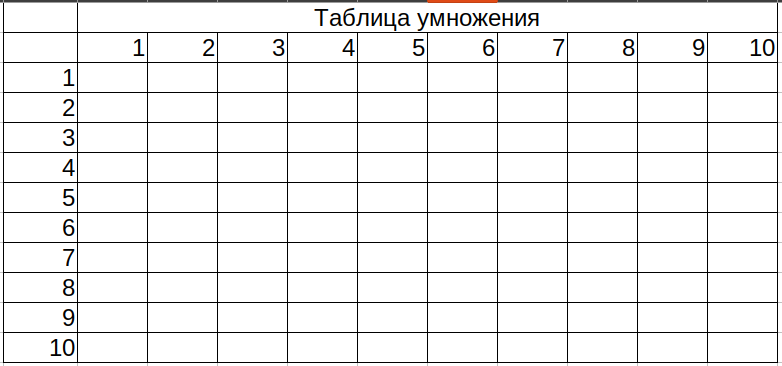
\includegraphics[width=\textwidth]{t1.png}

\subsubsection{Вычислить значения функции $y=\sin x$. Значения аргумента х изменяется от 0 до 10 с шагом 1. Постройте гладкий  график функции по таблице значений.}

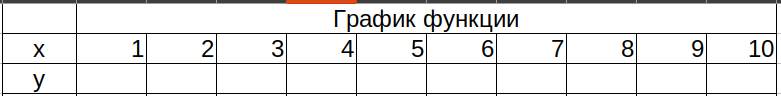
\includegraphics[width=\textwidth]{t2.png}

\subsubsection{Вычислить значения функции $x=16 * \sin^{3}t$ и $y = 13 * \cos(t) - 5 * \cos(2t) - 2 * \cos(3t) - \cos(4t)$. Значения аргумента x изменяется  от 0 до 6.4 с шагом 0.1. Постройте гладкий график функции по таблице значений}

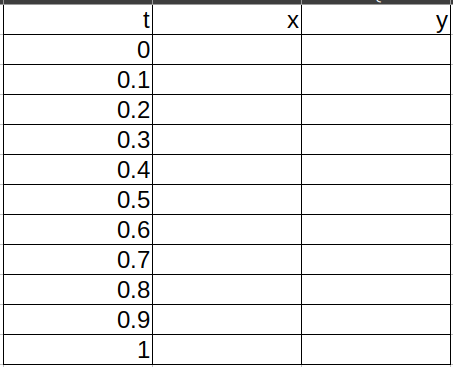
\includegraphics[width=\textwidth]{t3.png}

\subsubsection{}

\newpage
\subsection{Содержание отчета}
\begin{enumerate}
  \item Титульный Лист
  \item Цель работы
  \item Краткие теоретические сведения по теме лабораторной работы
  \item Выполненное задание
  \item Краткий вывод о проделанной работе
\end{enumerate}

\subsection{Литература}


\end{document}

\newpage
\section{Лабораторная работа №4. \newlineОсновы работы с базами данных}

Цель работы: Научиться создавать и использовать реляционные базы данных.

\subsection{Теоретические основы}

Хранение информации – одна из важнейших функций компьютера. Одним из распространенных средств такого хранения являются базы данных.\linebreak
\textbf{База данных (БД)} --- совокупность взаимосвязанных, хранящихся вместе данных при наличии такой минимальной избыточности, которая допускает их использование оптимальным образом для одного или нескольких приложений. Создание базы данных, ее поддержка и обеспечение доступа пользователей к ней осуществляется централизованно с помощью специального программного инструментария --- системы управления базами данных.\linebreak
\textbf{Система управления базами данных (СУБД)} --- это комплекс программных и языковых средств, необходимых для создания баз данных, поддержания их в актуальном состоянии и организации поиска в них необходимой информации. Концептуальная модель БД описывает сущности, их свойства и связи между ним и не зависит от конкретной СУБД.\linebreak
\textbf{Сущность} --- это реальный или представляемый тип объекта, информация о котором должна сохраняться и быть доступна. В диаграммах сущность представляется в виде прямоугольника, содержащего имя сущности. При этом имя сущности – это имя типа, а не некоторого конкретного экземпляра этого типа. Примеры сущностей: КАФЕДРА, ГРУППА, СТУДЕНТ. Каждый экземпляр сущности (объект) должен быть отличим от любого другого экземпляра той же сущности. Пример экземпляров сущности КАФЕДРА: КиПР, ЭГН, ТММСиИ, сущности СТУДЕНТ: Иванов А.П., Петрова Н.Н. \linebreak
\textbf{Связь} --- это ассоциация, устанавливаемая между двумя сущностями. Связь может существовать между двумя разными сущностями или между сущностью и ей же самой (рекурсивная связь). Возможны связи на основе отношений:
\begin{itemize}
    \item один-к-одному
    \item один-ко-многим
    \item многие-ко-многим
\end{itemize}

Связь «Один-ко-многим»: ГРУППА содержит много СТУДЕНТОВ. Каждый СТУДЕНТ входит только в одну ГРУППУ. Связь «Многие-ко-многим»: СОБАКА может укусить много ЧЕЛОВЕК, ЧЕЛОВЕК может быть укушен многими СОБАКАМИ. Связь "один к одному" встречается редко. Например, у нас есть таблица с информацией о всех сотрудниках и таблица с информацией о всех торговых агентах, которые являются сотрудниками нашего предприятия. Записи в таких таблицах могут быть связаны отношением "один к одному".

\subsubsection{Свойства сущностей}
Сущности имеют свойства, которые называются атрибутами.
Например, атрибуты:

сущности КАФЕДРА:
    \begin{itemize}
      \item название
      \item год создания
    \end{itemize}

сущности ГРУППА:
\begin{itemize}
    \item номер
    \item специальность
\end{itemize}

сущности СТУДЕНТ:
\begin{itemize}
\item фамилия
\item имя
\item отчество
\item номер студенческого билета
\item номер паспорта
\item год рождения
\item месяц рождения
\item день рождения
\end{itemize}

Любой атрибут принимает значения из некоторого множества допустимых значений, называемого доменом атрибута.

Например:
\begin{itemize}
  \item домен атрибута «год создания»: целые положительные числа;
    \item домен атрибута «имя»: строка, не содержащая пробелов;
    \item домен атрибута «год рождения»: целые положительные числа;
    \item домен атрибута «месяц рождения»: январь, февраль, март … декабрь;
    \item домен атрибута «день рождения»: целые числа от 1 до 31.
\end{itemize}

\subsubsection{Ключ сущности}

\textbf{Ключ сущности, первичный ключ} --- это атрибут (или множество атрибутов) уникальным образом идентифицирующих экземпляр сущности (объект). Например: ключ сущности СТУДЕНТ – номер студенческого билета, ключ КАФЕДРЫ --- название. Если ключ состоит из одного атрибута, его называют простым ключом. Если ключ сущности состоит из нескольких атрибутов, его называют составным ключом. Например, для сущности ДОМ с атрибутами «улица», «этажность», «год постройки», «номер дома», первичным ключом будет «улица»+ «номер дома».

\subsubsection{Реляционная модель данных}

Понятие реляционный (англ. relation --- отношение) связано с разработками известного американского специалиста в области систем баз данных Е.Кодда. Реляционная модель ориентирована на организацию данных в виде двумерных таблиц. Каждая реляционная таблица представляет собой двумерный массив и обладает следующими свойствами:

\begin{itemize}
    \item каждый элемент таблицы --- один элемент данных
    \item все столбцы в таблице однородные, т.е. все элементы в столбце имеют одинаковый тип (числовой, символьный и т.д.) и длину
    \item каждый столбец имеет уникальное имя (заголовки столбцов являются названиями полей в записях)
    \item одинаковые строки в таблице отсутствуют
  \item порядок следования строк и столбцов может быть произвольным
\end{itemize}

\textbf{Отношение} --- это плоская таблица, содержащая N столбцов, среди которых нет одинаковых. \textbf{N} --- это степень отношения, или арность отношения. Столбец отношения соответствует атрибуту сущности. \textbf{Кортеж} --- строка отношения (соответствует записи в таблице).

\textbf{Пример реляционной модели}

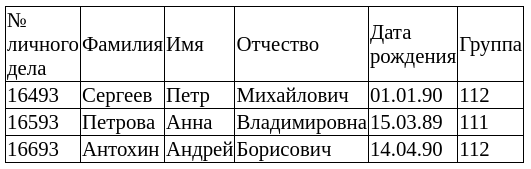
\includegraphics[width=\textwidth]{db1.png}

Отношения представлены в виде таблиц, строки которых соответствуют кортежам или записям, а столбцы --- атрибутам отношений, доменам, полям. Поле, каждое значение которого однозначно определяет соответствующую запись, называется простым ключом (ключевым полем). Если записи однозначно определяются значениями нескольких полей, то такая таблица базы данных имеет составной ключ. В примере ключевым полем таблицы является "№ личного дела".

\subsubsection{Нормализация}

\textbf{Нормальная форма} --- свойство отношения в реляционной модели данных, характеризующее его с точки зрения избыточности, потенциально приводящей к логически ошибочным результатам выборки или изменения данных. Нормальная форма определяется как совокупность требований, которым должно удовлетворять отношение. Процесс преобразования отношений базы данных к виду, отвечающему нормальным формам, называется нормализацией. Всего существует 8 нормальных форм, но мы рассмотрим только три, так как они редко рассматриваются в практическом проекте. Отсутствие учета этих правил может привести к меньшему созданию структуры базы данных, но не влияет на функциональность.

\textbf{Первая нормальная форма (1NF)} Переменная отношения находится в первой нормальной форме (1НФ) тогда и только тогда, когда в любом допустимом значении отношения каждый его кортеж содержит только одно значение для каждого из атрибутов.

\textbf{Вторая нормальная форма (2NF)} Переменная отношения находится во второй нормальной форме тогда и только тогда, когда она находится в первой нормальной форме и каждый неключевой атрибут неприводимо (функционально полно) зависит от её потенциального ключа. Функционально полная зависимость означает, что если потенциальный ключ является составным, то атрибут зависит от всего ключа и не зависит от его частей.

\textbf{Третья нормальная форма (3NF)} Переменная отношения находится в третьей нормальной форме тогда и только тогда, когда она находится во второй нормальной форме, и отсутствуют транзитивные функциональные зависимости неключевых атрибутов от ключевых.

Подробней процесс нормализации будет рассмотрен в практической части.
\subsection{Практическая часть}

LibreOffice Base позволяет создавать как локальные, так и сетевые реляционные базы данных или подключаться к уже имеющимся базам. В любом случае Base позволяет добавлять и удалять записи, редактировать данные, делать выборки, формировать отчеты.

\subsubsection{Создание базы данных}
При запуске LibreOffice Base предлагает создать новый файл базы данных или выбрать уже созданный, или подключится к существующей базе данных.

Для создания новой базы данных нужно выбрать первый пункт. Затем нажать Далее и выбрать Зарегистрировать базу данных и Открыть базу для редактирования. При завершении работы мастера потребуется указать имя новой базы и место для сохранения файла с ней. После этого открывается окно для работы с базой.

\begin{figure}[h]
\center{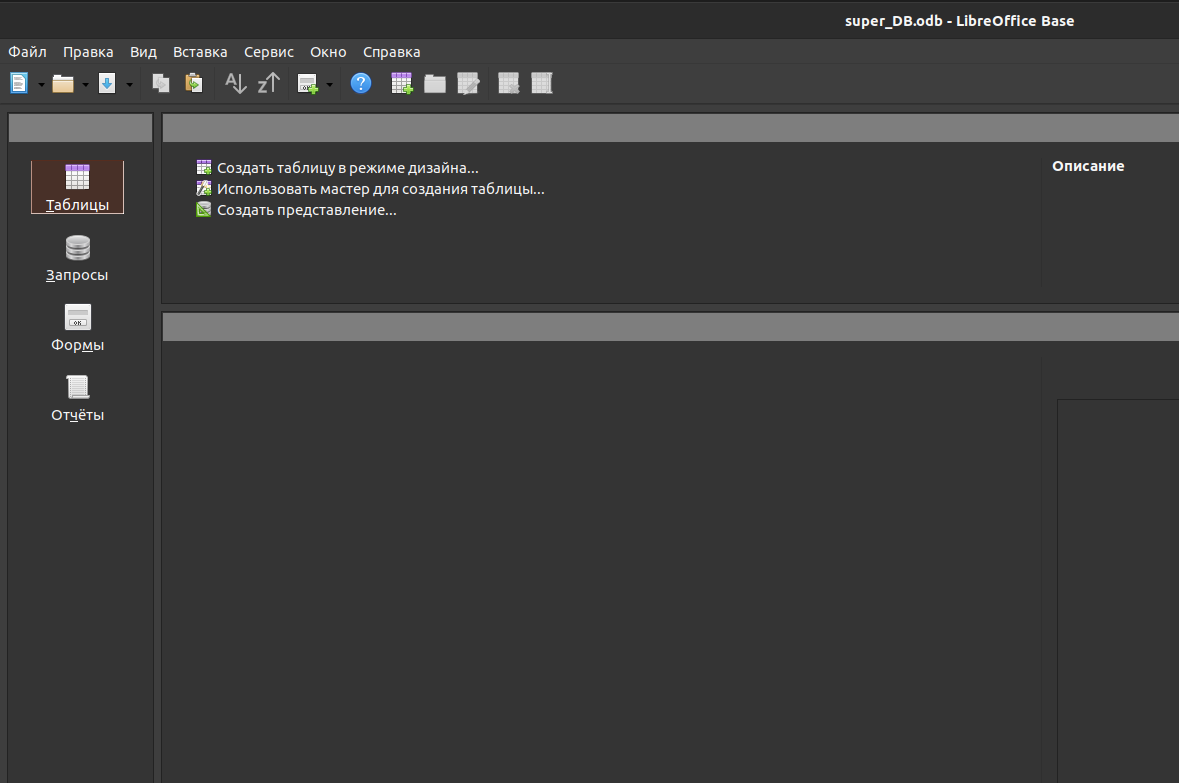
\includegraphics[width=\textwidth]{db2_main.png}
  \caption{Главное меню}\label{ris:main}}
\end{figure}

\subsubsection{Создание таблиц}

Во вкладке таблицы предоставляется выбор создания таблиц в дизайнере или по существующему шаблону с помощью мастера. Мы будем пользоватся дизайнером таблиц. При щелчке левой кнопкой мыши на элементе Таблицы, в правой нижней части рабочего поля будут перечислены имеющиеся таблицы, сейчас там пусто. В правой верхней части рабочего поля появляется набор возможных действий. Удобнее всего создавать таблицы в режиме дизайна. Для этого надо выбрать верхний пункт, после чего откроется соответствующее окно. Каждая строка окна Дизайнера таблиц (Table Disign) описывает одну колонку создаваемой таблицы. Первая строка Дизайнера соответствует первой колонке таблицы, вторая строка - второй колонке и так далее. На иллюстрации строки Дизайнера уже заполнены для создания конкретной таблицы. Проектирование таблицы --- ответственный этап создания базы данных. Ошибки, допущенные при проектировании таблицы потом сложно или вообще невозможно исправить.

При проектировании таблицы нужно обратить внимание на два основных момента. Перечень и порядок следования колонок определяют те данные об объекте, которые будут заноситься в базу и то, насколько удобно это будет делать. А свойства этих данных определяют размер файла базы. Это можно пояснить на примере показанной здесь таблицы студенты.

\begin{figure}[h]
\center{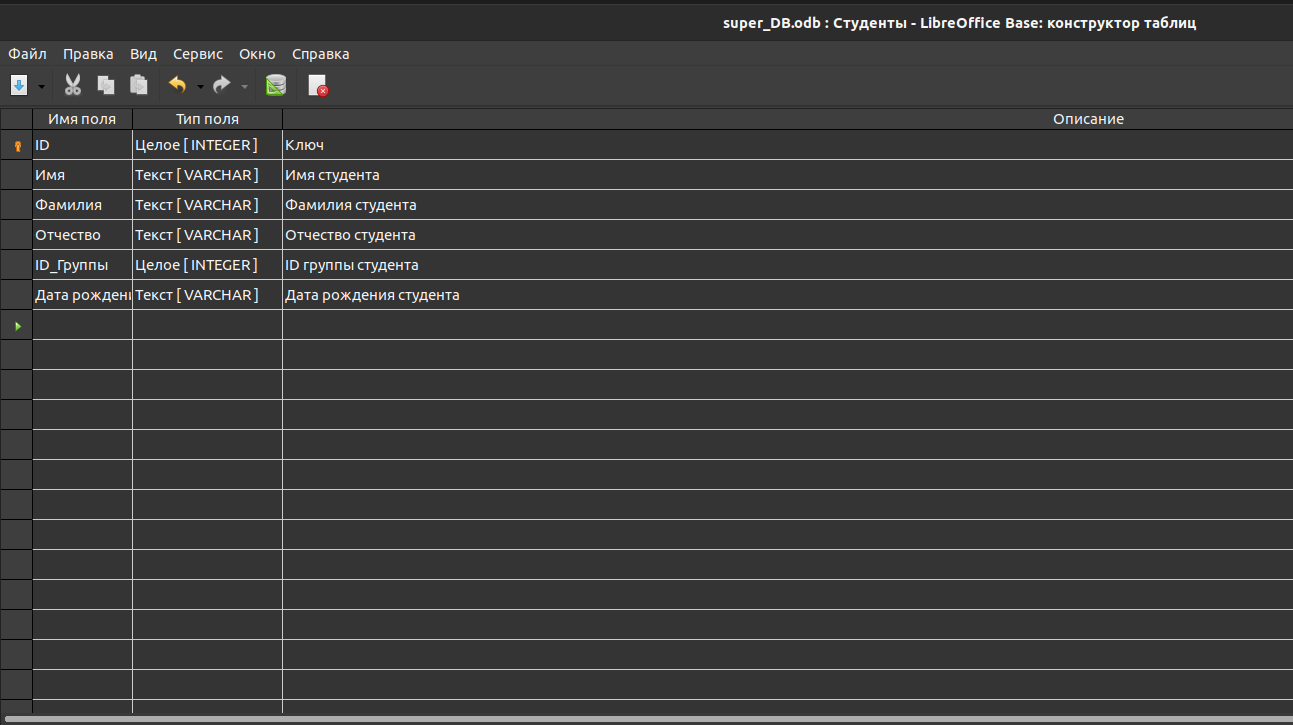
\includegraphics[width=\textwidth]{db3_construct.png}
  \caption{Создание таблицы}\label{ris:construct}}
\end{figure}

Каждая колонка таблицы имеет имя, которое задается в графе Имя поля. Хорошей практикой, особенно для таблиц с большим количеством колонок, является заполнение графы Описание. Тип поля заполняется путем выбора из вариантов, какого типа будет поле (текст, целые числа, дата).

Первая строка в таблице (ключ), является ключевым полем. Данные в ней будут появляться автоматически при добавлении каждой новой записи. Здесь это просто номер, который каждый раз увеличивается на единицу. Ключевое поле гарантирует, что в базе ни при каких обстоятельствах не будет содержаться двух одинаковых записей. Они обязательно будут отличаться друг от друга хотя бы ключом. Этого требует технология реляционных баз данных. Если ключевое поле не было создано, Дизайнер обратит на это внимание и предложит его создать.

\newpage
\subsubsection{Нормализация}
Для примера рассмотрим базу данных студентов, таблица \ref{tab:0NF}

\textbf(1NF) --- В первой нормальной форме все значения в ячейках (их в теории называют атрибуты) должны быть атомарными, то есть содержать ровно одно неделимое значение, а не список из нескольких значений. Например в таблице \ref{tab:0NF} атрибуты с информацией о студенте находятся не в атомарном состоянии. Из-за этого нам нелегко, например, сделать выборку студентов по группе. Для решения проблемы необходимо вынести информацию о группе и телефоне в отдельные колонки. Также, возможно, имеет смысл разбить ФИО на 3 отдельных колонки, но это зависит от того, как они будут использоваться - всегда вместе или по отдельности.

\begin{table}[h]
      \caption{Не нормализованная таблица}
      \begin{center}\label{tab:0NF}
        %\toprule
      \begin{tabular}{|c|c|}
        \hline
        Студенты & Информация \\
        \hline
        Иванов Иван Иванович & Б20-111, 8655655656\\
        Петров Петр петрович & Б20-111, 89566766545\\
        Сергеев Сергей Сергеевич & Б20-222, 8656554343\\
        Георгиев Георгий Георгиевич & Б20-222, 8765676654\\
        Афанасьев Афанасий Афанасиевич & Б20-333, 8765432123\\
        \hline
      \end{tabular}
    \end{center}
  \end{table}

\noindent После изменения получилась таблица \ref{tab:1NFDONE} удовлетворяющая условиям первой нормальной форме. Теперь все атрибуты находятся в атомарном состояниии что позволяет легко совершать поиск и редактирование по таблице.

\begin{table}[h]
      \caption{1NF}
      \begin{center}\label{tab:1NFDONE}
        %\toprule
      \begin{tabular}{|c|c|c|c|c|}
        \hline
        Фамилия & Имя & Отчество & Телефон & Группа\\
        \hline
        Иванов & Иван & Иванович & 89677656554 & Б20-111\\
        Петров & Петр & Петрович & 87654567876 & Б20-111\\
        Сергеев & Сергей & Сергеевич & 8976787654 & Б20-222\\
        Георгиев & Георгий & Георгиевич & 9876543212 & Б20-222\\
        Афанасьев & Афанасий & Афанасиевич & 89908767656 & Б20-333\\
        \hline
      \end{tabular}
    \end{center}
  \end{table}

\noindent \textbf(2NF) --- во второй нормальной форме все поля в таблице должны полностью зависеть от первичного ключа целиком, а не от его части. Обычно это требование применяется только тогда, когда первичный ключ составной и содержит 2 или больше колонок. В этом случае, если какие-то значения в таблице зависят только от части ключа, то они могут повторяться, и их надо вынести в отдельную таблицу. Если первичный ключ - это одно поле, то таблица уже соответствует требованию. Поэтому таблица \ref{tab:1NFDONE} уже находится во второй нормальной форме так как все поля зависят от ее первичного ключа 'Телефон'. Но если появится студенты у которых нет телефона то правило уникальности ключа будет нарушено, поэтому стоит добавить исусственный ключ - ID студента.

\begin{table}[h]
      \caption{2NF}
      \begin{center}\label{tab:2NFDONE}
        %\toprule
      \begin{tabular}{|c|c|c|c|c|c|}
        \hline
        ID & Фамилия & Имя & Отчество & Телефон & Группа\\
        \hline
        1 & Иванов & Иван & Иванович & 89677656554 & Б20-111\\
        2 & Петров & Петр & Петрович & 87654567876 & Б20-111\\
        3 & Сергеев & Сергей & Сергеевич & 8976787654 & Б20-222\\
        4 & Георгиев & Георгий & Георгиевич & 9876543212 & Б20-222\\
        5 & Афанасьев & Афанасий & Афанасиевич & 89908767656 & Б20-333\\
        \hline
      \end{tabular}
    \end{center}
  \end{table}

  \noindent \textbf(3NF) --- в третьей нормальной форме значения полей должны зависеть только от первичного ключа, а не от других полей. В таблице \ref{tab:2NFDONE} видно что названия групп повторяются и не зависят от первичного ключа. Например, когда потребуется переименовать название группы то придется изменить названия в каждой строке таблицы. Это значит что поле ``Группа'' нужно вывести из этой таблицы в отдельную таблицу.

  \begin{table}[h]
      \caption{3NF-Студенты}
      \begin{center}\label{tab:3NFDONE_STUDENTS}
        %\toprule
      \begin{tabular}{|c|c|c|c|c|c|}
        \hline
        ID & Фамилия & Имя & Отчество & Телефон & IDГруппа\\
        \hline
        1 & Иванов & Иван & Иванович & 89677656554 & 1\\
        2 & Петров & Петр & Петрович & 87654567876 & 1\\
        3 & Сергеев & Сергей & Сергеевич & 8976787654 & 2\\
        4 & Георгиев & Георгий & Георгиевич & 9876543212 & 2\\
        5 & Афанасьев & Афанасий & Афанасиевич & 89908767656 & 3\\
        \hline
      \end{tabular}
    \end{center}
  \end{table}

\begin{table}[h]
      \caption{3NF-Группы}
      \begin{center}\label{tab:3NFDONE_GROUPS}
        %\toprule
      \begin{tabular}{|c|c|}
        \hline
        ID & Группа\\
        \hline
        1 & Б20-111\\
        2 & Б20-222\\
        3 & Б20-333\\
        \hline
      \end{tabular}
    \end{center}
  \end{table}

В итоге нормализации получились две таблицы отвечающие требованию третьей нормальной формы.

\subsubsection{Наполнение таблиц}
Созданные таблицы отображаются во вкладке Таблицы главного меню. Если нажать на значек таблицы откроется окно ввода данных. Таблицы заполняются вручную или импортируются из заранее подготовленной электронной таблицы. Пример заполненой таблицы на рис.\ref{ris:tabins}

\begin{figure}[h]
\center{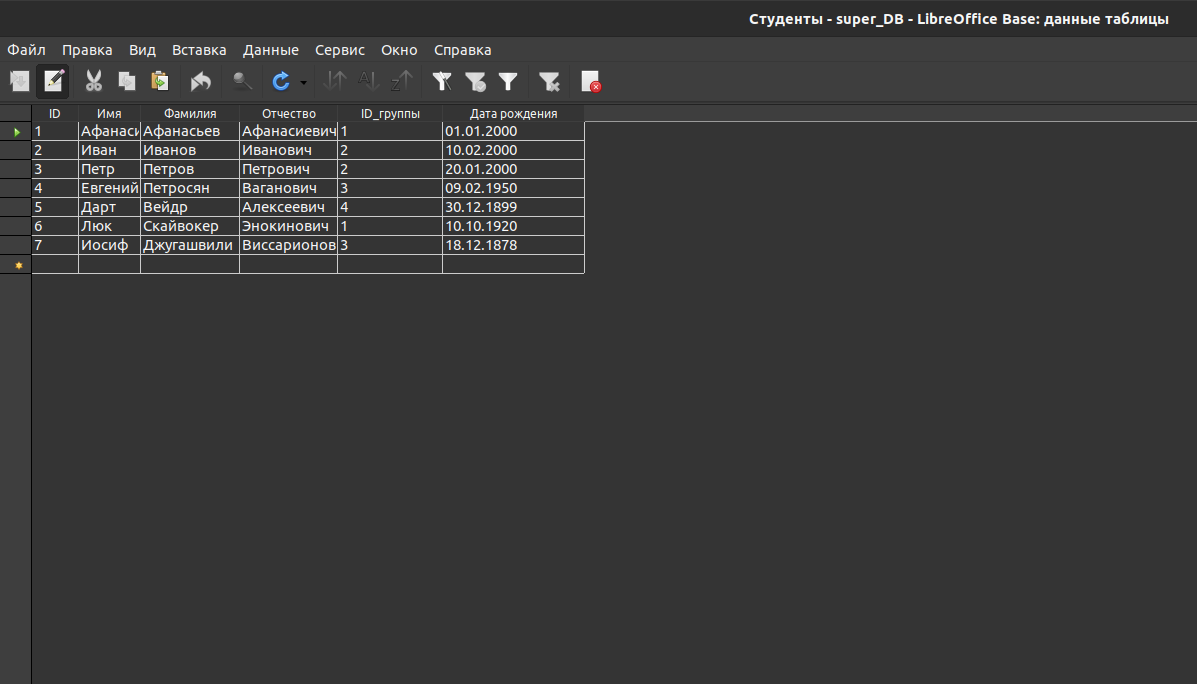
\includegraphics[width=\textwidth]{db_tabins.png}
  \caption{Таблица студенты}\label{ris:tabins}}
\end{figure}

\subsubsection{Создание запросов}

\textbf{Запрос (query)} --- это средство выбора необходимой информации из базы данных. Применяются два типа запросов: по образцу QBE и структурированный язык запросов SQL.

\textbf{QBE – Query by example} – средство для отыскания необходимой информации в базе данных. Он формируется не на специальном языке, а путем заполнения бланка запроса в окне Конструктора запросов.

\textbf{SQL --- Structured Query Language} --- это запросы, которые составляются (программистами) из последовательности SQL --- инструкций. Эти инструкции задают, что надо сделать с входным набором данных для генерации выходного набора.

Существует несколько типов запросов: на выборку, на обновление, на добавление, на удаление, перекрестный запрос, создание таблиц. Наиболее распространенным является запрос на выборку. Запросы на выборку используются для отбора нужной пользователю информации, содержащейся в таблицах. Они создаются только для связанных таблиц.

Так как для ипользования SQL потребуется дополнительные знания синтаксиса языка и понимание основ программирования, \textbf{можно использовать QBE}. Но стоит заметить что SQL имеет большую выразительную силу, и позволет быстрее описать желаемый результат. Далее в примерах будет использоватся SQL.

Для создания запросов необходимо перейти во кладку запросы и выбрать Создать запрос в режиме SQL. После того как запрос будет написан, необходимо нажать на значек выполнить запрос или нажать на клавишу F5. LibreOffice Base обработает запрос и вернет результат Рис. \ref{ris:selection}.

\begin{figure}[h]
\center{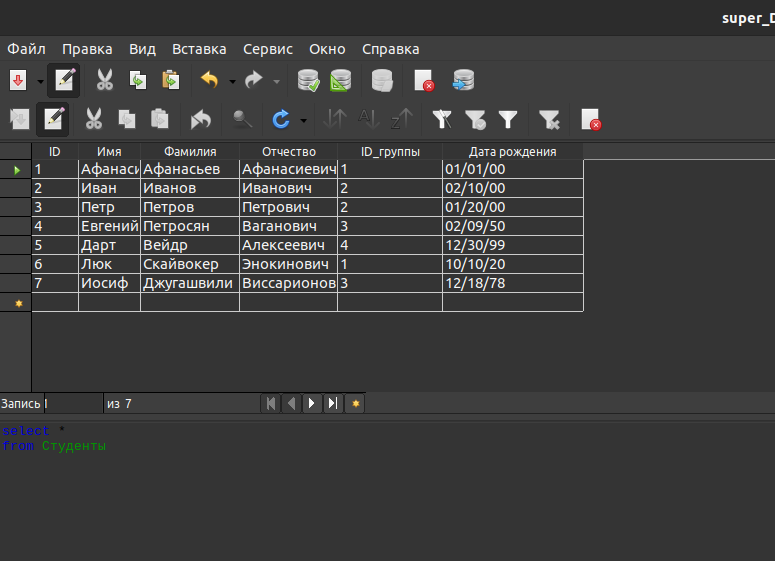
\includegraphics[width=\textwidth]{db_selection.png}
  \caption{Таблица студенты}\label{ris:selection}}
\end{figure}

\newpage
\begin{lstlisting}[label=select, caption=Базовая структура запроса]
SELECT
  [DISTINCT | DISTINCTROW | ALL]
  select_expression,...
FROM table_references
[WHERE where_definition]
[GROUP BY {unsigned_integer | col_name | formula}]
[HAVING where_definition]
[ORDER BY {unsigned_integer | col_name | formula} [ASC | DESC], ...]
\end{lstlisting}

\begin{lstlisting}[label=selection,caption=Выборка всех студентов]
  select *
  from Студенты
\end{lstlisting}

Ключевое слово \textbf{select} определяет список возвращаемых столбцов (как существующих, так и вычисляемых), их имена, ограничения на уникальность строк в возвращаемом наборе, ограничения на количество строк в возвращаемом наборе. Знак звезда (*) обозначает выборку всех столбцов результата запроса. Ключевое слово \textbf{from} задаёт табличное выражение, которое определяет базовый набор данных для применения операций, определяемых в других предложениях оператора т.е. указывает из каких таблиц делать выборку.

\newpage
\begin{lstlisting}[label=where, caption=Выборка студентов с датой рождения большей или равной условию]
  select *
  from Студенты
  where ДатаРождения >= {d '1950-02-01' }
\end{lstlisting}

\noindent\textbf{where} - оператор в SQL, указывающий, запрос должен действовать только на записи,
удовлетворяющие определенным критериям. Критерии должны быть описаны в форме предикатов. Раздел WHERE — не обязательный раздел в SQL запросах. Он используется в качестве условия в SQL-запросе для ограничения записей обрабатываемых в выражениях SQL или возвращаемых запросом. В листинге \ref{where} оператор where задает условие выборки при котором должны отображатся только те студенты у которых день рождения больше или равно 1950.02.01. Для сравнения типа данных дата, в LibreOffice Base используются формат \{d 'ГГГГ-ММ-ДД'\}.


\begin{lstlisting}[label=order, caption=Запрос фамилий и дат рождения студентов отсортированных по дате рождения]
  select Фамилия, ДатаРождения
  from Студенты
  order by ДатаРождения desc
\end{lstlisting}

\noindent\textbf{order by} --- необязательный параметр оператора SELECT, который означает что запрос ,возвращают набор строк, отсортированных по значениям одного или более столбцов. Его можно применять как к числовым столбцам, так и к строковым. В последнем случае, сортировка будет происходить по алфавиту. Использование предложения ORDER BY является единственным способом отсортировать результирующий набор строк. Без этого предложения СУБД может вернуть строки в любом порядке. Если упорядочение необходимо, ORDER BY должен присутствовать в SELECT. Сортировка может производиться как по возрастанию, так и по убыванию значений. Параметр \textbf{ASC} (по умолчанию) устанавливает порядок сортировки по возрастанию, от меньших значений к большим. Параметр \textbf{DESC} устанавливает порядок сортировки по убыванию, от больших значений к меньшим.

\begin{lstlisting}[label=group, caption=Запрос количества телефонов у студентов]
select Фамилия, count( Телефон. НомерТелефона)
from Студенты, Телефон
where  Студенты.ID = Телефон.  ID студента
group by Фамилия
\end{lstlisting}

\noindent\textbf{group by} --- необязательный параметр операторa SELECT, для группировки строк по результатам агрегатных функций (MAX, SUM, AVG, COUNT, ...). Необходимо, чтобы в SELECT были заданы только требуемые в выходном потоке столбцы, перечисленные в GROUP BY и/или агрегированные значения. Распространённая ошибка — указание в SELECT столбца, пропущенного в GROUP BY.

\begin{lstlisting}[label=group, caption=Запрос количества телефонов у студентов]
select Фамилия, count( Телефон. НомерТелефона)
from Студенты, Телефон
where  Студенты.ID = Телефон.  ID студента
group by Фамилия
\end{lstlisting}

\newpage
\subsection{Задание на лабораторную работу}

Для выполнения работы необходимо:
\begin{enumerate}
  \item Изучить теоретический материал
  \item Выбрать задание в соответствии с вариатом
  \item Продумать предметную область
  \item Создать базу данных
  \item Разработать таблицы с учетом нормализации (3NF)
  \item Наполнить таблицы данными (минимум 10 строк)
   \item Создать 5 запросов:
    \begin{itemize}
      \item Выборка всех данных
      \item Выборка с условием
      \item Выборка с сортировкой
      \item Выборка с агрегатной функцией
      \item Выборка с условием на результат агрегатных функций (having)
    \end{itemize}
  \item Оформить отчет по лабораторной работе
\end{enumerate}

\textbf{Перечень вариантов:}

\begin{enumerate}
  \item Спроектировать БД для задачи «Оплаты за электроэнергию», которая содержит следующую:
    \begin{itemize}
      \item ФИО ответственного квартиросъемщика
      \item Номер лицевого счета
      \item Название месяца
      \item Стоимость 1 КВт/ч
      \item Кол-во израсходованной в месяц электроэнергии
      \item Сумма к оплате
    \end{itemize}


  \item Спроектировать БД для задачи «Учет выдачи пенсий», которая содержит следующую информацию:
    \begin{itemize}
        \item ФИО пенсионера
        \item Адрес
        \item Название месяца
        \item Способ выдачи пенсии
        \item Дата получения
        \item Сумма пенсии
    \end{itemize}

  \item Спроектировать БД для задачи «Учет выдачи канцтоваров по отделам», которая содержит следующую информацию:
    \begin{itemize}
        \item ФИО работника
        \item Должность
        \item Отдел
        \item Название канцтоваров
        \item Количество
        \item Дата выдачи
\end{itemize}

  \item Спроектировать БД для задачи «Учет оборудования отдела», которая содержит следующую информацию :
    \begin{itemize}
        \item ФИО ответственного
        \item Отдел
        \item Наименование оборудования
        \item Количество
        \item Дата получения
    \end{itemize}

  \itemСпроектировать БД для задачи «Учет выполненных работ», которая содержит следующую информацию :
    \begin{itemize}
        \item ФИО работника
        \item Должность
        \item Наименование работы
        \item Срок выполнения
        \item Дата получения
        \item Отметка о выполнении
    \end{itemize}

  \item Спроектировать БД для задачи «Учет заказов», которая содержит следующую информацию:
    \begin{itemize}
        \item ФИО покупателя
        \item Наименование товара
        \item Дата заказа
        \item Способ доставки
        \item Дата получения
        \item Стоимость товара
    \end{itemize}

  \item Разработать БД администратора ателье по ремонту оргтехники. БД должна вести учет:
    \begin{itemize}
        \item Клиентов ателье
        \itemТехники, сданной в ремонт
        \item Проделанной работы
        \item Работников ателье
    \end{itemize}

  \item Разработать БД администратора автосалона. БД должна вести учет:
    \begin{itemize}
        \item Автомобилей, находящихся в автосалоне
        \item Роставщиков автомобилей
        \item Клиентов автосалона
        \item Поставок
        \item Заказов
    \end{itemize}

  \item Агенство занимается продажей авиабилетов на различные рейсы, ведет учет проданных билетов и учет пассажиров, купивших билеты. БД должна содержать следующие данные:
    \begin{itemize}
        \item информация о расписании рейсов
        \item информация о свободных местах
        \item информация о пассажирах, купивших билеты на рейс
        \item информация о выполненном рейсе
    \end{itemize}

  \item Спроектировать базу данных фирмы «Мебель», хранящую информацию:
    \begin{itemize}
        \item об изделиях
        \item о мастерах
        \item о клиентах фирмы
        \item накладные, составляемые при отгрузке изделий клиентам
    \end{itemize}


  \item Спроектировать базу данных по производству обуви. База данных должна хранить данные:
    \begin{itemize}
        \item о каждом сотруднике
        \item список поставщиков продукции
        \item о комплектующих
        \item данные о каждом поставщике
        \item список выполняемых сотрудниками работ.
    \end{itemize}


  \item Разработать БД администратора ресторана. БД должна вести учет:
    \begin{itemize}
        \item распределения столиков
        \item клиентов ресторана
        \item предварительных заказов на столики
        \item меню
        \item заказов на конкретный столик
    \end{itemize}

  \item Разработать БД сотрудника ЖЭС (ЖЭС – жилищно-эксплуатационная служба). БД должна вести учет:
    \begin{itemize}
        \item всех домов, подчиняющихся ЖЭС
        \item квартиросъемщиков
        \item стоимости всех услуг ЖЭС
        \item льготных квартиросъемщиков ЖЭС
        \item стоимости оплаты за квартиру
      \item задолжников по оплате (начисление пени)
    \end{itemize}

  \item Разработать БД «Университет», содержащую следующую информацию:
    \begin{itemize}
        \item о преподавателе;
        \item о дисциплинах;
        \item о заведующих кафедрой;
        \item кабинет, где преподаватель читает свои предметы
    \end{itemize}


  \item Разработать БД «Поликлиника». БД должна содержать информацию:
    \begin{itemize}
        \item о пациенте;
        \item текущее состояние пациента;
        \item о лечащем враче;
        \item диагноз, поставленный пациенту
    \end{itemize}


\end{enumerate}

\subsection{Содержание отчета}
\begin{enumerate}
  \item Титульный Лист
  \item Цель работы
  \item Краткие теоретические сведения по теме лабораторной работы
  \item Выполненное задание
  \item Краткий вывод о проделанной работе
\end{enumerate}

\begin{thebibliography}{3}
  \bibitem{Mich1}
Минченков, И. Н. Практическая работа с базами данных в OpenOffice.org Base : учебное пособие / И.
Н. Минченков. — Липецк : Липецкий государственный технический университет, ЭБС АСВ, 2012. — 49 c. — ISBN 978-5-88247-534-4. — Текст : электронный // Электронно-библиотечная система IPR BOOKS : [сайт]. — URL: http://www.iprbookshop.ru/17704.html (дата обращения: 26.10.2020).
\bibitem{bd2}
Базы данных : учебное пособие / . — Саратов : Научная книга, 2012. — 158 c. — ISBN 2227-8397. — Текст : электронный // Электронно-библиотечная система IPR BOOKS : [сайт]. — URL: http://www.iprbookshop.ru/6261.html (дата обращения: 26.10.2020).
\end{thebibliography}


\end{document}
